\section{Introduction to the Amateur Radio Service}
\label{sec:intro_amateur_radio}

The Amateur Radio Service, often referred to as ham radio, is a popular hobby and service that brings people, electronics, and communication together. It is a unique blend of technical skill, public service, and international camaraderie. This section introduces the fundamental concepts of the Amateur Radio Service, including its purpose, regulatory framework, and key definitions.

\subsection*{Basis and Purpose of the Amateur Radio Service}
The Amateur Radio Service is governed by a set of principles and purposes that guide its operation. According to the Federal Communications Commission (FCC), the primary purpose of the Amateur Radio Service is to advance skills in the technical and communication phases of the radio art. This includes fostering experimentation, improving technical proficiency, and providing a pool of trained operators who can assist in times of emergency. The service also promotes international goodwill by allowing operators to communicate across borders.

\subsection*{Regulatory Authority of the FCC}
The FCC is the primary regulatory body responsible for overseeing the Amateur Radio Service in the United States. The FCC establishes and enforces the rules that govern amateur radio operations, ensuring that the service operates in the public interest. These rules are codified in Title 47 of the Code of Federal Regulations, Part 97 (FCC Part 97). The FCC also maintains the Universal Licensing System (ULS), a database that contains information about all licensed amateur radio operators and stations.

\begin{figure}[ht]
    \centering
    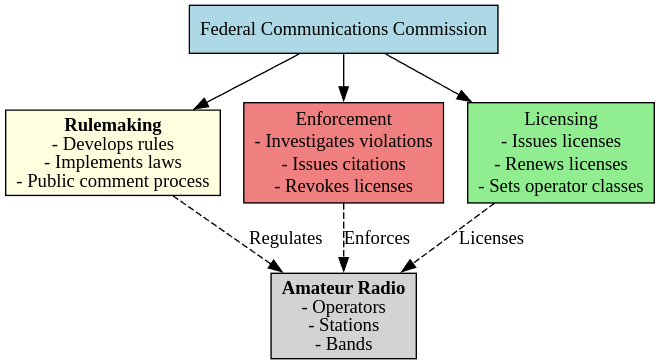
\includegraphics[width=0.8\textwidth]{tech/organized/chapter_1/images/fcc_structure.png}
    \caption{FCC Regulatory Structure}
    \label{fig:fcc_structure}
    % Diagram showing the structure of the FCC and its role in amateur radio regulation. The diagram should include the FCC at the top, with branches for rulemaking, enforcement, and licensing. Arrows should indicate the flow of authority and responsibility.
\end{figure}


\subsection*{Phonetic Alphabet Usage}
The use of a phonetic alphabet is encouraged in the Amateur Radio Service, particularly for station identification. The phonetic alphabet helps to ensure clarity and accuracy in communication, especially when dealing with weak signals or noisy conditions. While not mandatory in all situations, its use is a best practice that enhances the effectiveness of amateur radio communications.

\begin{table}[ht]
    \centering
    \begin{tabular}{|l|l||l|l||l|l|}
        \hline
        A & Alpha & J & Juliet & S & Sierra \\
        B & Bravo & K & Kilo & T & Tango \\
        C & Charlie & L & Lima & U & Uniform \\
        D & Delta & M & Mike & V & Victor \\
        E & Echo & N & November & W & Whiskey \\
        F & Foxtrot & O & Oscar & X & X-ray \\
        G & Golf & P & Papa & Y & Yankee \\
        H & Hotel & Q & Quebec & Z & Zulu \\
        I & India & R & Romeo & & \\
        \hline
    \end{tabular}
    \caption{NATO Phonetic Alphabet}
    \label{tab:phonetic_alphabet}
\end{table}

\subsection*{License Grants and Documentation}
An individual may hold only one operator/primary station license grant at any given time. This license is documented in the FCC ULS database, which serves as the official record of the license grant. The appearance of the license in the ULS database is the definitive proof that the FCC has issued the license. Printed copies or email notifications are not considered official documentation.

\subsection*{Definitions of Beacon and Space Station}
FCC Part 97 provides specific definitions for key terms used in the Amateur Radio Service. A \textit{beacon} is defined as an amateur station that transmits communications for the purposes of observing propagation or related experimental activities. A \textit{space station}, on the other hand, is an amateur station located more than 50 km above Earth's surface. These definitions are important for understanding the scope and limitations of amateur radio operations.

\subsection*{Questions}

\begin{tcolorbox}[colback=gray!10!white,colframe=black!75!black,title={T1A01}]
    Which of the following is part of the Basis and Purpose of the Amateur Radio Service?
    \begin{enumerate}[label=\Alph*),noitemsep]
        \item Providing personal radio communications for as many citizens as possible
        \item Providing communications for international non-profit organizations
        \item \textbf{Advancing skills in the technical and communication phases of the radio art}
        \item All these choices are correct
    \end{enumerate}
\end{tcolorbox}
The Basis and Purpose of the Amateur Radio Service, as defined by the FCC, includes advancing skills in the technical and communication phases of the radio art. This is the primary goal of the service, making option C correct. Options A and B are not part of the official basis and purpose.

%memory_trick T1A01

\begin{tcolorbox}[colback=gray!10!white,colframe=black!75!black,title={T1A02}]
    Which agency regulates and enforces the rules for the Amateur Radio Service in the United States?
    \begin{enumerate}[label=\Alph*),noitemsep]
        \item FEMA
        \item Homeland Security
        \item \textbf{The FCC}
        \item All these choices are correct
    \end{enumerate}
\end{tcolorbox}
The Federal Communications Commission (FCC) is the agency responsible for regulating and enforcing the rules for the Amateur Radio Service in the United States. This is clearly stated in FCC Part 97.

%memory_trick T1A02

\begin{tcolorbox}[colback=gray!10!white,colframe=black!75!black,title={T1A03}]
    What do the FCC rules state regarding the use of a phonetic alphabet for station identification in the Amateur Radio Service?
    \begin{enumerate}[label=\Alph*),noitemsep]
        \item It is required when transmitting emergency messages
        \item \textbf{It is encouraged}
        \item It is required when in contact with foreign stations
        \item All these choices are correct
    \end{enumerate}
\end{tcolorbox}
The FCC encourages the use of a phonetic alphabet for station identification, but it is not mandatory in all situations. This practice helps to ensure clear communication, especially under challenging conditions.

%memory_trick T1A03

\begin{tcolorbox}[colback=gray!10!white,colframe=black!75!black,title={T1A04}]
    How many operator/primary station license grants may be held by any one person?
    \begin{enumerate}[label=\Alph*),noitemsep]
        \item \textbf{One}
        \item No more than two
        \item One for each band on which the person plans to operate
        \item One for each permanent station location from which the person plans to operate
    \end{enumerate}
\end{tcolorbox}
An individual may hold only one operator/primary station license grant at any given time. This is a fundamental rule in the Amateur Radio Service.

%memory_trick T1A04

\begin{tcolorbox}[colback=gray!10!white,colframe=black!75!black,title={T1A05}]
    What proves that the FCC has issued an operator/primary license grant?
    \begin{enumerate}[label=\Alph*),noitemsep]
        \item A printed copy of the certificate of successful completion of examination
        \item An email notification from the NCVEC granting the license
        \item \textbf{The license appears in the FCC ULS database}
        \item All these choices are correct
    \end{enumerate}
\end{tcolorbox}
The official proof of an operator/primary license grant is its appearance in the FCC ULS database. Printed copies or email notifications are not considered official documentation.

%memory_trick T1A05

\begin{tcolorbox}[colback=gray!10!white,colframe=black!75!black,title={T1A06}]
    What is the FCC Part 97 definition of a beacon?
    \begin{enumerate}[label=\Alph*),noitemsep]
        \item A government transmitter marking the amateur radio band edges
        \item A bulletin sent by the FCC to announce a national emergency
        \item A continuous transmission of weather information authorized in the amateur bands by the National Weather Service
        \item \textbf{An amateur station transmitting communications for the purposes of observing propagation or related experimental activities}
    \end{enumerate}
\end{tcolorbox}
A beacon, as defined by FCC Part 97, is an amateur station that transmits communications for the purposes of observing propagation or related experimental activities. This definition is specific to the Amateur Radio Service.

%memory_trick T1A06

\begin{tcolorbox}[colback=gray!10!white,colframe=black!75!black,title={T1A07}]
    What is the FCC Part 97 definition of a space station?
    \begin{enumerate}[label=\Alph*),noitemsep]
        \item Any satellite orbiting Earth
        \item A manned satellite orbiting Earth
        \item \textbf{An amateur station located more than 50 km above Earth's surface}
        \item An amateur station using amateur radio satellites for relay of signals
    \end{enumerate}
\end{tcolorbox}
A space station, according to FCC Part 97, is an amateur station located more than 50 km above Earth's surface. This definition distinguishes space stations from other types of amateur stations.

%memory_trick T1A07

\subsection*{Summary}
This section introduced the Amateur Radio Service, its purpose, and the regulatory framework established by the FCC. Key concepts include:

\begin{itemize}
    \item \textbf{Purpose of the Amateur Radio Service}: Advancing technical and communication skills, fostering experimentation, and providing emergency communications.
    \item \textbf{Regulatory authority of the FCC}: The FCC regulates and enforces the rules for amateur radio operations in the United States.
    \item \textbf{Phonetic alphabet usage}: Encouraged for clear and accurate station identification.
    \item \textbf{License grants and documentation}: Only one operator/primary station license grant is allowed per person, and the license must appear in the FCC ULS database.
    \item \textbf{Definitions of beacon and space station}: A beacon is an amateur station for propagation observation, while a space station is located more than 50 km above Earth's surface.
\end{itemize}
